\label{chapt:prelim}

The analysis process is discussed

\section{Simplifications}

The results were simplified to do.

%Example of using an equation and refering to it
\subsection{Equations}


The first equation that is presented , Equation~\ref{eq:eqnstatics}

% First equation of basic statics
\begin{equation}
	\label{eq:eqnstatics}
	% must use aligned to get multi line equation	
	\begin{aligned}
		\Sigma F_i=0 \\
		\Sigma M_i=0 
	\end{aligned}
\end{equation}


As per reference \cite{timoshenko1959theory}

%Example of using table
\subsection{Table}

This was used to get the results in the following Table~\ref{table:testtbl}.
	
\begin{table}[ht]
	\caption{Test table 1}
	\centering
	\begin{tabular}{c c c}
		%heading
		\hline \hline  Case & Method \#1 & Method \#2 \\[0.5ex]
		\hline
		%Main table body content	
		1                   & 10         & 50         \\
		2                   & 20         & 100        \\ [1ex]
		\hline
	\end{tabular}
	\label{table:testtbl}
\end{table}


\section{Theory of Cylindrical Shells}

As per Timoshenko's book INSERT REF, this section will cover the method of approximating the cylinder as a long thin shell. The following coordinate system is presented as per Figure~\ref{fig:CoordSyst} below.

\begin{figure}[!htbp]
	\centering
	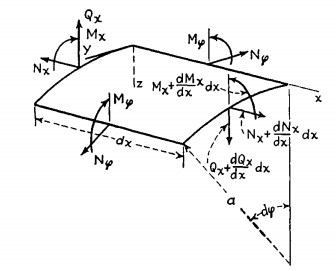
\includegraphics[width=0.6\textwidth]{CoordSyst}
	\caption{Coordinate system adopted for derivation of DEs.}
	\label{fig:CoordSyst}
\end{figure}

Based on this, the following differential equations are presented as a pressure balance knowing that the differential area can be represented as Equation~\ref{eq:diffsurf}
 
\begin{equation}
	\label{eq:diffsurf}
	dA = dS\ dx = a\ d\varphi \ dx   
\end{equation}

The equations of equilibrium may be written as a force projection about the x and z axis and momment balance about y as Equations ~\ref{eq:eqbrm_x}, ~\ref{eq:eqbrm_z}, ~\ref{eq:eqbrm_y} respectively.

\begin{equation}
	\label{eq:eqbrm_x}
	\frac{dN_x}{dx}\ a\ d\varphi \ dx = 0
\end{equation}

\begin{equation}
	\label{eq:eqbrm_z}
	\frac{dQ_x}{dx}\ a\ d\varphi \ dx+ N_\varphi \ a\ d\varphi \ dx +Z\ a\ d\varphi \ dx= 0
\end{equation}

\begin{equation}
	\label{eq:eqbrm_y}
	\frac{dM_x}{dx}\ a\ d\varphi \ dx- Q_x\ a\ d\varphi \ dx= 0
\end{equation}

First looking at \ref{eq:eqbrm_x}, simplifying this equation and taking the integral with respect to $x$ will leave \ref{eq:eqbrm_x2}. 

\begin{equation}
	\label{eq:eqbrm_x2}
	N_x = C = 0 
\end{equation}

This above equation simply states that the effects of bending due to the axial forces will be neglected.\\

Similarly with \ref{eq:eqbrm_z} and \ref{eq:eqbrm_y}, simplifications will lead to \ref{eq:eqbrm_z2} and \ref{eq:eqbrm_y2} respectively.
\begin{equation}
	\label{eq:eqbrm_z2}
	\frac{dQ_x}{dx}+\frac{1}{a}\ N_\varphi = -Z
\end{equation}

\begin{equation}
	\label{eq:eqbrm_y2}
	\frac{dM_x}{dx}- Q_x= 0
\end{equation} 

With these equations and using strain relations from Hooke's law, the fine DE for displacement will be determined. In Equation ~\ref{eq:strain_xphi}, the relations between displacement and strain are presented.

\begin{equation}
	\label{eq:strain_xphi}
	\begin{aligned}
		\epsilon_x = \frac{du}{dx}      \\
		\epsilon_\varphi = -\frac{w}{a} 
	\end{aligned}
\end{equation}

From Hooke's law $N_x$ may be also written as Equation~\ref{eq:Hookes_Nx}. Substituting ~\ref{eq:strain_xphi} will leave the final simplification.
\begin{equation}
	\label{eq:Hookes_Nx}
	N_x = \frac{Eh}{1-\nu^2}\ \left( \epsilon_x + \nu \epsilon_\varphi \right) =  \frac{Eh}{1-\nu^2}\ \left( \frac{du}{dx} -\nu \ \frac{w}{a} \right)
\end{equation} 

%%tilde is UNBREAKABLE SPACE
Solving Equation~\ref{eq:Hookes_Nx} using ~\ref{eq:eqbrm_x2} leaves \ref{eq:Nx_simpl}.
\begin{equation}
	\label{eq:Nx_simpl}
	\frac{du}{dx} =  \nu \ \frac{w}{a}
\end{equation} 

Similarly, with $N_\varphi$, again applying \ref{eq:strain_xphi} leaves \ref{eq:Nphi_simpl}.
\begin{equation}
	\label{eq:Hookes_Nphi}
	N_\varphi = \frac{Eh}{1-\nu^2}\ \left( \epsilon_\varphi + \nu \epsilon_x \right) = \frac{Eh}{1-\nu^2}\  \left( -\frac{w}{a}+\nu \ \frac{du}{dx} \right)
\end{equation} 

\begin{equation}
	\label{eq:Nphi_simpl}
	N_\varphi = - \frac{Ehw}{a}
\end{equation}

 
